%%%%%%%%%%%%%%%%%%%%%%%%%%%%%%%%%%%%%%%%%%%%%%%%%%%%%%%%%%%%%%%%%%%%%%%%%%%%%%%%
%2345678901234567890123456789012345678901234567890123456789012345678901234567890
%        1         2         3         4         5         6         7         8
\documentclass[letterpaper, 10 pt, conference]{ieeeconf}  % Comment this line out
% if you need a4paper
%\documentclass[a4paper, 10pt, conference]{ieeeconf}      % Use this line for a4

\usepackage{float}
% paper
% uso paquete bookmark para tener bien los outlines.
\usepackage{bookmark}

% Configuro el idioma.
\usepackage[utf8]{inputenc} % Importante para mantener acentos.
\usepackage[spanish, activeacute]{babel} % Requiere: texlive-lang-spanish. Por primera vez hay que ejecutar: texconfig init> log

% Paquete para poder usar acentos en $$.
\usepackage{mathtools}
%\setmathfont{XITS math}

\usepackage{tikz}
\usetikzlibrary{shapes.misc, positioning, shapes.geometric, arrows.meta}

\usepackage{siunitx}

% package to get \url
\usepackage{hyperref}
\hypersetup{
  colorlinks=true,
  linkcolor=magenta,
  filecolor=magenta,
  citecolor=magenta,      
  urlcolor=magenta,
}

% Graficos electrónicos
\usepackage{circuitikz}

\IEEEoverridecommandlockouts                              % This command is only
% needed if you want to
% use the \thanks command
\overrideIEEEmargins
% See the \addtolength command later in the file to balance the column lengths
% on the last page of the document

\usepackage{graphicx}
\usepackage{graphics}

% styling for matlab/octave code.
\usepackage{matlab-prettifier}
% Configuracion, con esto puede agregar ñ.
\lstset{
  literate={ñ}{{\~n}}1
}

% The following packages can be found on http:\\www.ctan.org
%\usepackage{graphics} % for pdf, bitmapped graphics files
%\usepackage{epsfig} % for postscript graphics files
%\usepackage{mathptmx} % assumes new font selection scheme installed
%\usepackage{times} % assumes new font selection scheme installed
\usepackage{amsmath} % assumes amsmath package installed
%\usepackage{amssymb}  % assumes amsmath package installed

\title{\LARGE \bf Laboratorio N° 2}

\author{
  Tom\'as Vidal\\
  {\it Circuitos Electrónicos 1}\\
  {\it Facultad de Ingenier\'ia, UNLP, La Plata, Argentina.}\\
  {\it 15 de Mayo, 2024.}
}                                            % <-this % stops a space


% comienzo

% INTRO

% Figura
\newcommand{\image}[2] {
  \begin{figure}[H]
    \centering
    \includegraphics[width=0.43\textwidth]{./#1.png}
    \caption{#2}
    \label{fig:#1}
  \end{figure}
}

% Codigo
% \begin{lstlisting}[style=Matlab-editor]
% % el código va aca
% dispc("HELLO WORLD");
% \end{lstlisting}

\begin{document}
\maketitle
\thispagestyle{empty}
\pagestyle{empty}

\section{INTRODUCCCI\'ON}
% TODO

\section{Comportamiento de los operacionales}
\subsection{Topologías}
Se emplearon las siguientes configuraciones de los amplificadores operacionales.
\begin{figure}[H]
  \centering
  \begin{circuitikz}
    \node[op amp] (opamp) at (0,0) {};
    \draw (opamp.+) -- ++(0,-1) to[R=$1k$] ++(0,-1.5) node[ground]{};
    \draw (opamp.-) -- ++(-1,0) to[R=$1k$] ++(-1.25,0) -- ++(-0.5,0) node[ocirc]{} coordinate (Vin) node[left] {$+V_{in}$};
    \draw (opamp.out) -- ++(0.25,0) -- ++(0,2) -- ++(-0.5,0) to[R=$10k$] ++(-2.5,0) -- ++(0,-1.5) node[circ](node_oa-){};
    \draw (opamp.out) -- ++(0.25,0) node[circ](node_out){} -- ++(0.25,0) node[ocirc]{} coordinate (Vout) node[right] {$+V_{out}$};
    \draw (node_oa-) ++(0,1.5) node[circ]{}  -- ++(0,1.5) -- ++(0,0) to[C=$10nF$] ++(3,0) -- ++(0,-1.5) node[circ]{};
  \end{circuitikz}
  \caption{Amplificador operacional en configuración de integrador}
  \label{diagAOIntegrador}
\end{figure}
\begin{figure}[H]
  \centering
  \begin{circuitikz}
    \node[op amp] (opamp) at (0,0) {};
    \draw (opamp.+) -- ++(-0.5,0) -- ++(0,-0.5) to[R=$1k$] ++(0,-1.5) node[ground]{};
    \draw (opamp.-) -- ++(0,0) to[R=$1k$] ++(-2,0) -- ++(0,0) to[C=$10nF$] ++(-0.5,0) -- ++(-0.5,0) node[ocirc]{} coordinate (Vin) node[left] {$+V_{in}$};
    \draw (opamp.out) -- ++(0,0) -- ++(0,2) -- ++(-0.5,0) to[R=$10k$] ++(-2,0) -- ++(0,-1.5) node[circ]{};
    \draw (opamp.out) -- ++(0,0) node[circ]{} -- ++(0.25,0) node[ocirc]{} coordinate (Vout) node[right] {$+V_{out}$};
  \end{circuitikz}
  \caption{Amplificador operacional en configuración de derivador}
  \label{diagAODerivador}
\end{figure}
Las mismas tienen las siguientes trasferencias:
\begin{itemize}
  \item \textbf{Integrador:} 
    \begin{equation} \label{eq:integrador_trans}
      \frac{V_{salida}}{V_{entrada}} = \frac{10}{\frac{s}{10k} + 1}
    \end{equation}
  \item \textbf{Derivador:} 
    \begin{equation} \label{eq:derivador_trans}
      \frac{V_{salida}}{V_{entrada}} = \frac{-100\mu s}{ \frac{s}{100k} + 1}
    \end{equation}
\end{itemize}

En la ec. \ref{eq:integrador_trans} se puede observar que hay un polo en $s=0$, y en la ec. \ref{eq:derivador_trans} hay un polo en $s=10k$. Estos polos nos dan una noción de las limitaciones de los circuitos, más aún sabiendo que en la realidad no se puede sintetizar el polo en el origen, solo uno lo suficientemente ``cerca'' del origen tal que se comporte como un integrador para las frecuencias deseadas. Por lo tanto solo hay un rango de frecuencias para las cuales estos circuitos se comportarán como se esperan. Para el integrador siempre que la frecuencia de operación teórica sea mayor a $10kHz$ el circuito se comportará como un integrador, de otra manera el polo dominante hace que se comporte como un inversor. Para el caso del derivador 
\subsection{Resultados de las topologías}
Lo observado experimentalmente concuerda con lo que se explicó previamente. Si se inyectaba una señal menor a $10kHz$ el integrador se actúaba como un inversor, pero para frecuencias lo suficientemente elevadas integraba la señal de entrada correctamente

\textit{En las siguientes fotos las señales de color amarillo son las señales de entrada y las de color azul las salida}

\begin{figure}[H]
  \centering
  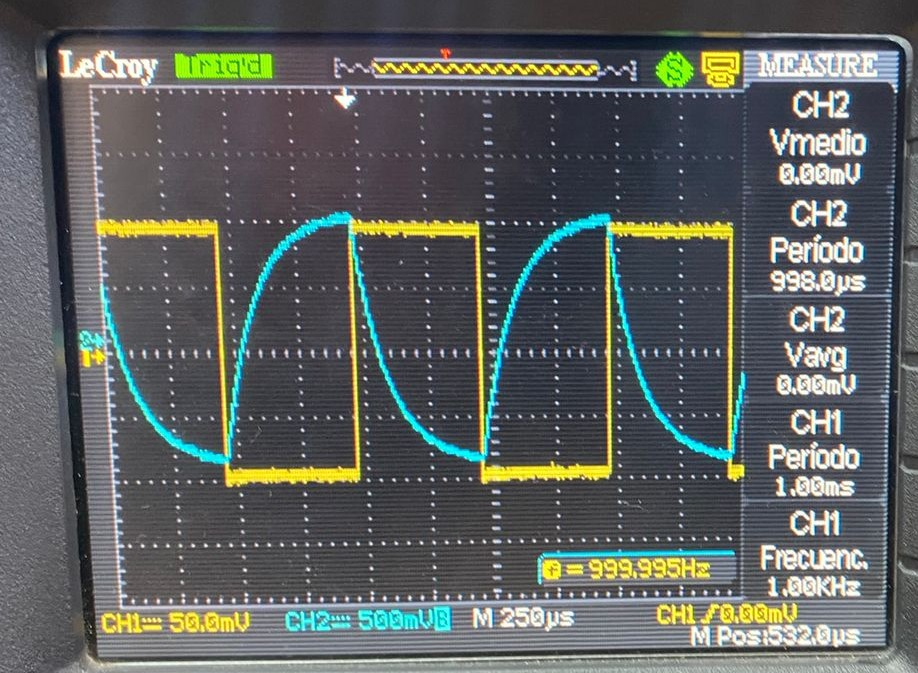
\includegraphics[width=0.43\textwidth]{./Imagenes/integrador_1khz.jpeg}
  \caption{Integrador en mala zona de operación (1kHz)}
  \label{pic:int_1khz}
\end{figure}

\begin{figure}[H]
  \centering
  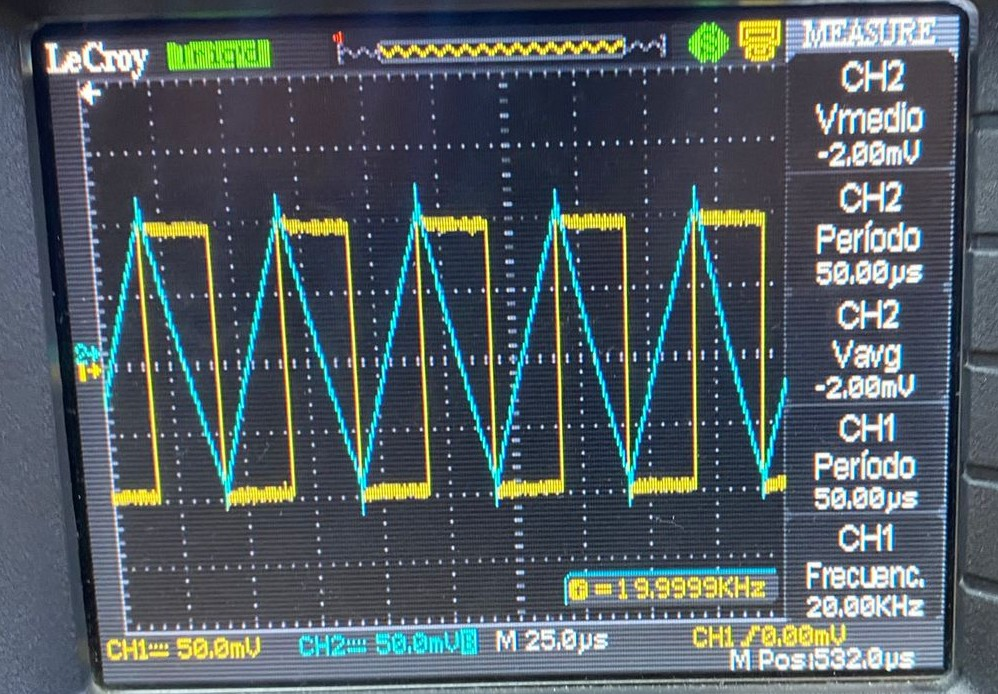
\includegraphics[width=0.43\textwidth]{./Imagenes/integrador_20khz.jpeg}
  \caption{Integrador en buena zona de operación (20kHz)}
  \label{pic:int_20khz}
\end{figure}

En la foto \ref{pic:int_1khz} se ve que la salida se distorsiona (la integral del cajón es un triángulo), pero en la foto \ref{pic:int_20khz} hay triángulos perfectos, lo que verifica lo explicado previamente.


\begin{figure}[H]
  \centering
  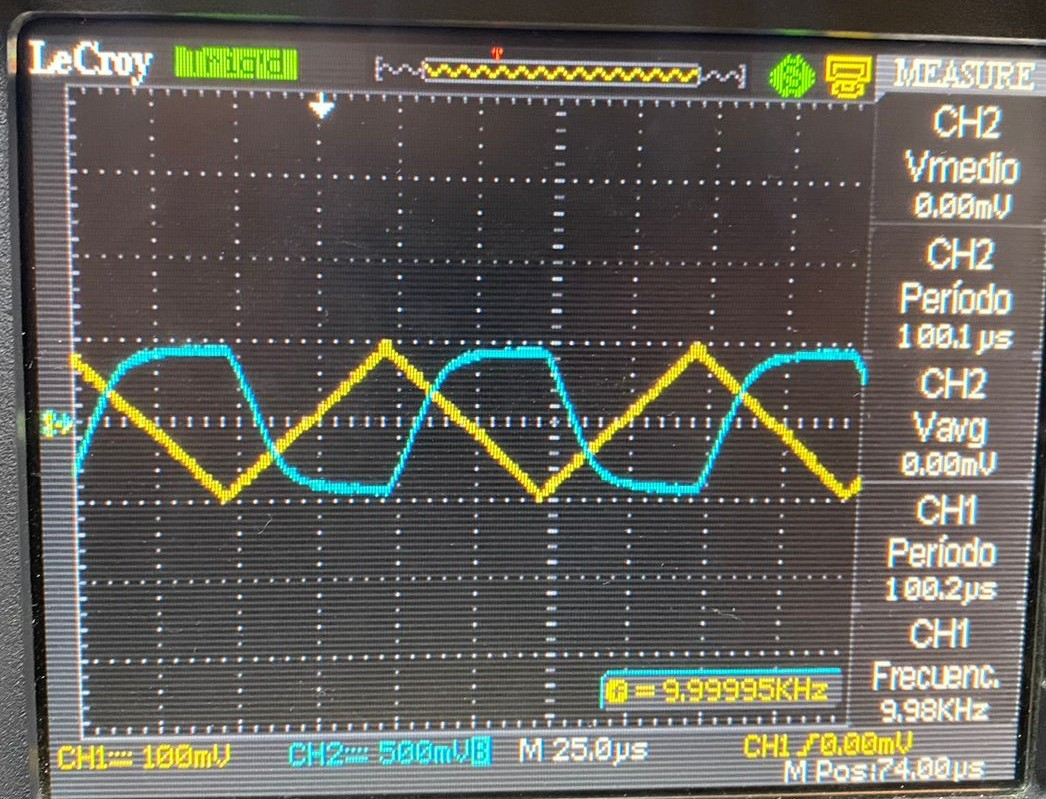
\includegraphics[width=0.43\textwidth]{./Imagenes/derivador_10khz.jpeg}
  \caption{Derivador en mala zona de operación (10kHz)}
  \label{pic:der_10khz}
\end{figure}

\begin{figure}[H]
  \centering
  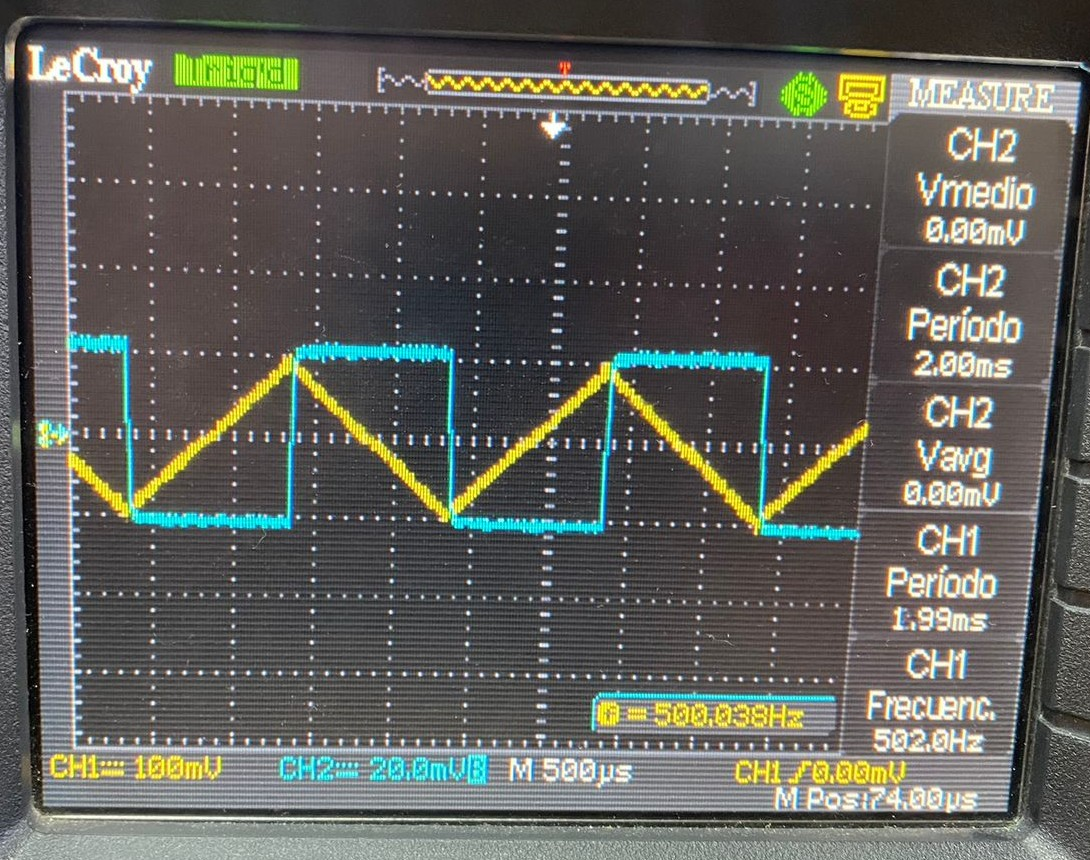
\includegraphics[width=0.43\textwidth]{./Imagenes/derivador_500hz.jpeg}
  \caption{Integrador en buena zona de operación (500Hz)}
  \label{pic:der_500hz}
\end{figure}

Para el derivador se ve en la foto \ref{pic:der_10khz} como la señal de salida se distorsiona (cuando se deriva un triángulo se obtiene un cajón), ya que está operando en $10kHz$, en cambio, para un frecuencia de $500Hz$ funciona correctamente como se observa en la foto \ref{pic:der_500hz}.

\section{Circuito sumador/comparador}
En el segundo circuito provisto (\ref{fig:diag-top-2}) se puede concluir (a través de un análisis por etapas de amplificación) que es un sumador de dos señales, de las cuales una es invertida previamente ($V_{1}$), además al final el resultado es amplificado (con ganancia dependiente de la frecuencia). En esencia este circuito es un \textbf{comparador} con ganancia en función de la frecuencia.
\begin{figure}[H]
  \centering
  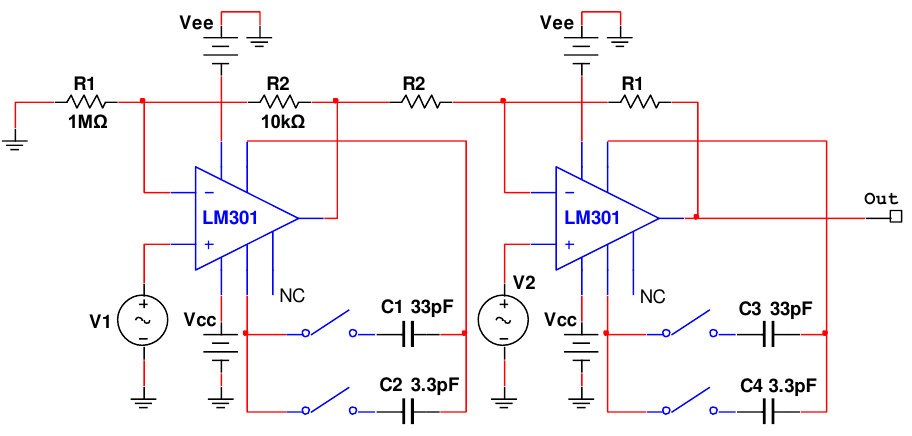
\includegraphics[width=0.43\textwidth]{./Imagenes/topologia2.png}
  \caption{Diagrama esquemático de la segunda topología}
  \label{fig:diag-top-2}
\end{figure}
\begin{figure}[H]
  \centering
  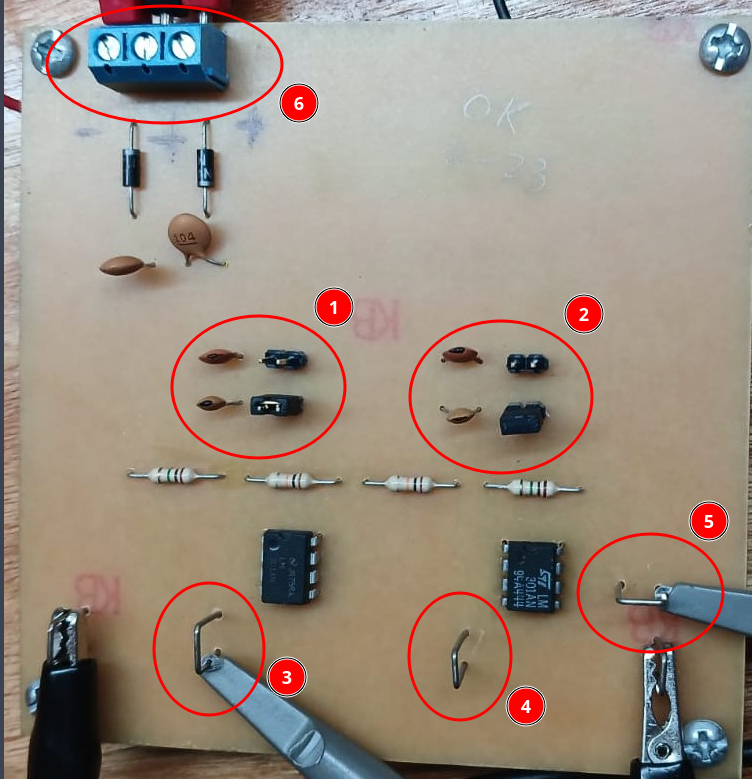
\includegraphics[width=0.43\textwidth]{./Imagenes/topologia2_placa.png}
  \caption{Placa de circuitos provista de la segunda topología}
  \label{pic:topologia2_placa}
\end{figure}

En la placa de la figura \ref{pic:topologia2_placa} las indicaciones 1 y 2 refieren a los capacitores de compensación, que se pueden ajustar como lo indica el diagrama esquemático \ref{fig:diag-top-2}, las indicaciones 3 y 4 son las señales de entrada, y la salida es la 5. La alimentación es la 6

\begin{figure}[H]
  \centering
  \begin{tikzpicture}[auto, node distance=2cm, thick]
    % Define block styles
    \tikzstyle{block} = [rectangle, draw, minimum height=2em, minimum width=2em, align=center]
    \tikzstyle{sum} = [circle, draw, inner sep=0pt, minimum size=3em, node distance=2cm]
    \tikzstyle{line} = [-, thick]
    \tikzstyle{triangle} = [regular polygon, regular polygon sides=3, draw, minimum size=1.5em, shape border rotate=270, align=center]
    % Blocks and nodes
    \node [block] (S1) {$V_1$};
    \node [triangle, right=.5cm of S1] (neg) {-1};
    \node [sum, right=.5cm of neg] (sum) {+};
    \node [block, below=.5cm of sum] (S2) {$V_2$};
    \node [triangle, right=.5cm of sum] (g) {g(f)};
    \node [block, right=.4cm of g] (output) {Salida};

    % Connections
    \draw[-Stealth] (S1) -- (neg);
    \draw[-Stealth](neg) -- (sum);
    \draw[-Stealth](S2) -- (sum);
    \draw[-Stealth](sum) -- (g);
    \draw[-Stealth](g) -- ++(1,0) -- ++(0.5,0);

  \end{tikzpicture}

  \caption{Diagrama en bloques del comparador}
  \label{diag:comparador}
\end{figure}

\subsection{Sin señales de entrada}
Cuando se mide la salida del circuito sin señales de entrada (es decir las entradas quedan ``flotando''), tanto con capacitores de ajuste o sin los mismos, se observa ruido en la salida, lo que es de esperar ya que el ruido que proviene de las entradas es amplificado por las diferentes etapas.
\begin{figure}[H]
  \centering
  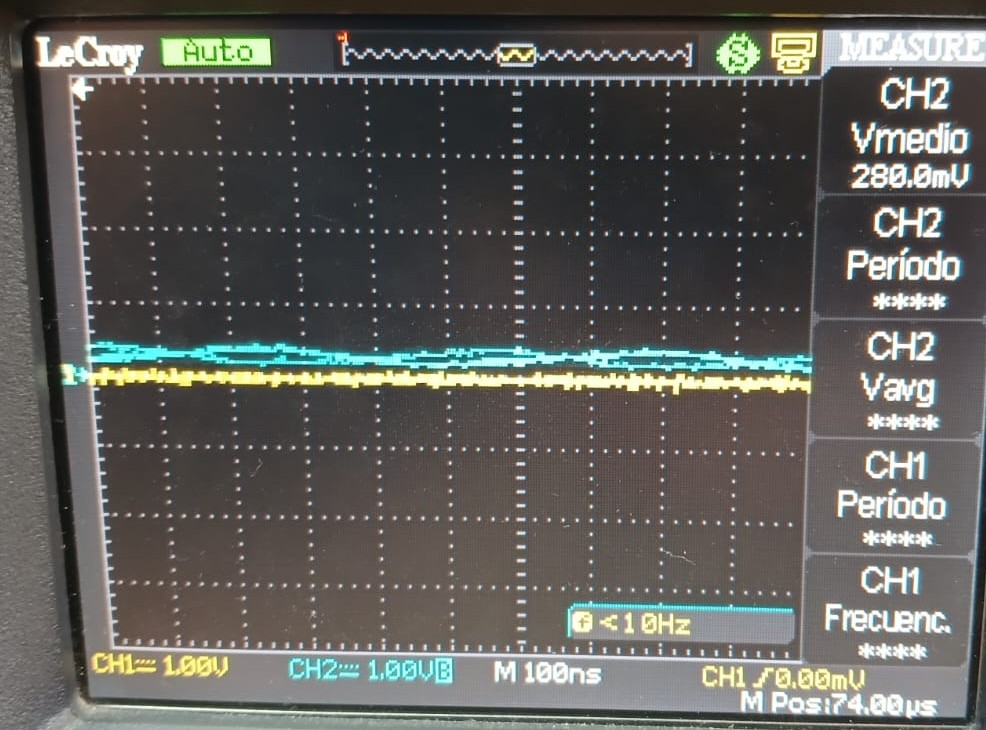
\includegraphics[width=0.43\textwidth]{./Imagenes/sin_entradas.jpeg}
  \caption{Segunda placa sin señales de entradas}
  \label{pic:sin_entradas}
\end{figure}

\subsection{Con señal V1}
Se inyectó una señal sinusoidal en $V_{1}$ de amplitud 20mV y frecuencia 100Hz, en $V_{2}=0$. En la salida se obtuvo una sinusoidal de 100hz desfasada en 180 grados y de amplitud 2V, que es acorde a lo esperado ya $Salida=g(f)*( V_{2} - V_{1} )=100*(-V_{1})$
\begin{figure}[H]
  \centering
  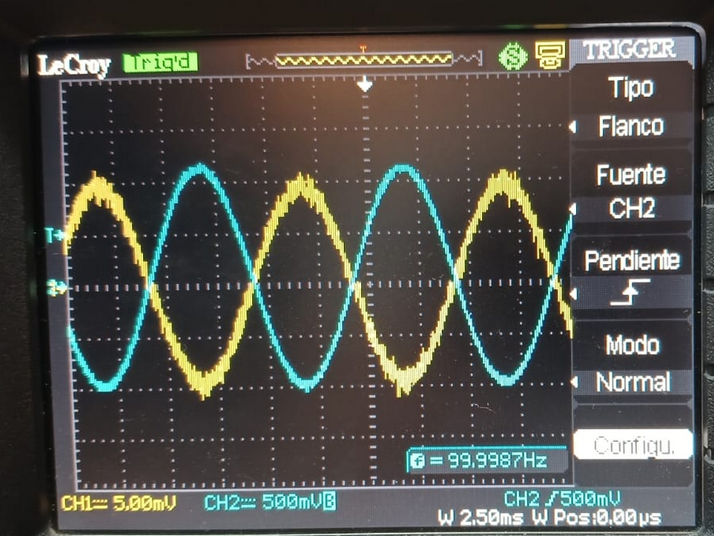
\includegraphics[width=0.43\textwidth]{./Imagenes/v1_100hz.png}
  \caption{Segunda placa sin señales de entradas}
  \label{pic:100hz_v1}
\end{figure}

\subsection{Con señal V2}
Se inyectó una señal sinusoidal en $V_{2}$ de amplitud 20mV y frecuencia 100Hz, en $V_{1}=0$. En la salida se obtuvo una sinusoidal de 100hz y de amplitud 2V, que es acorde a lo esperado puesto que $Salida=g(f)*( V_{2} - V_{1} )=100*(V_{2})$ (es decir que no hay desfase entre la entrada y la salida).
\begin{figure}[H]
  \centering
  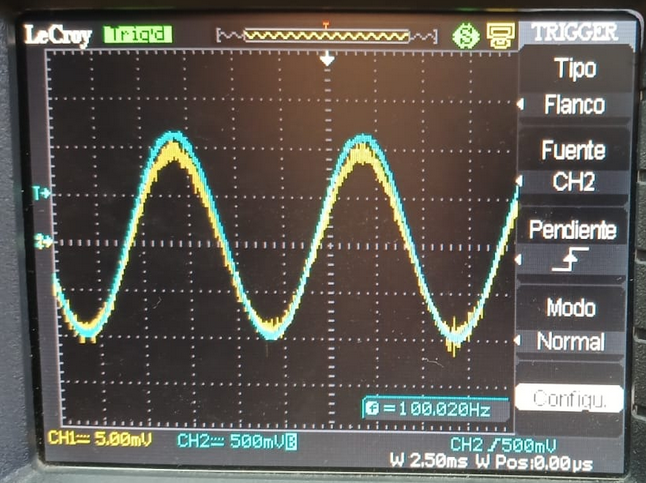
\includegraphics[width=0.43\textwidth]{./Imagenes/v2_100hz.png}
  \caption{Segunda placa sin señales de entradas}
  \label{pic:100hz_v2}
\end{figure}

\subsection{Frecuencias de corte}
Se hizo un barrido en frecuencia para ambas posiciones de los \textit{jumpers} (capacitores de 3.3pF y 33pF). Para el polo dominante para los capacitores de 3.3pF fue de 27kHz, y para los de 33pF fue de 8.5kHz aproximadamente.
\begin{table}[H]
  \centering
  \begin{tabular}{|l|l|l|}
    \hline
    Capacitores (pF)  & Polo dominante (KHz)  \\ \hline
    3.3               & 27                    \\ \hline
    33                & 8.5                   \\ \hline
  \end{tabular}
  \caption{Resultados de los barridos en frecuencia}
  \label{tab:result_barr_frec}
\end{table}

\subsection{Entradas en modo común}
Se conectaron en paralelo las entradas $V_{1}$ y $V_{2}$, y a las mismas se les inyectó una señal sinusoidal de 100Hz y amplitud 20mV. A la salida se obtuvo 


\end{document}
